\documentclass{beamer}
\usepackage{multicol}
\usepackage{natbib} 
\usepackage{amsmath}
\usepackage{amsfonts}
\def\newblock{\hskip .11em plus .33em minus .07em}
\newcommand\independent{\protect\mathpalette{\protect\independenT}{\perp}} 
\def\independenT#1#2{\mathrel{\rlap{$#1#2$}\mkern2mu{#1#2}}} 
\newcommand{\field}[1]{\mathbb{#1}}

%\usepackage{beamerthemeBerkeley}
% Use either the one above or the one below
\usetheme{Hannover}

\title{Potential Outcomes and Causal Effects}
%\author{	F. Daniel Hidalgo\\ }
%\date{\today}

\begin{document}

\frame{\titlepage}

%\section[Outline]{}
%\frame{\tableofcontents}
\section{Neyman (1923)} % (fold)
\label{sec:neyman_1923_}

% section neyman_1923_ (end)
\begin{frame}[t]\frametitle{Neyman}
	\begin{figure}[htbp]
		\centering
			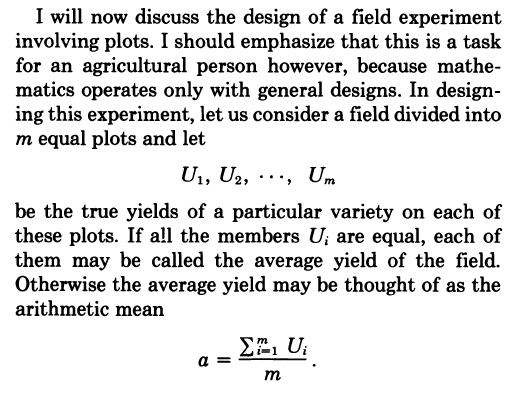
\includegraphics[height=3in]{neyman1.png}
		\label{fig:neyman1}
	\end{figure}
	
\end{frame}

\begin{frame}[t]\frametitle{Neyman}
	\begin{figure}[htbp]
		\centering
			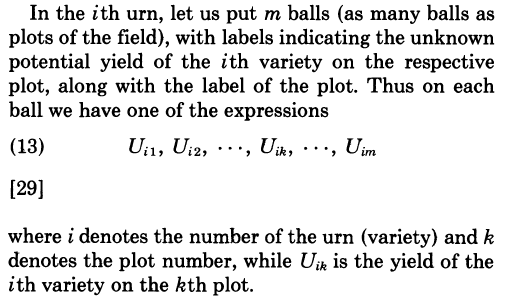
\includegraphics[height=2.5in]{neyman2.png}
		\label{fig:neyman2}
	\end{figure}
	
\end{frame}

\begin{frame}[t]\frametitle{Disappearing Balls}
	\begin{figure}[htbp]
		\centering
			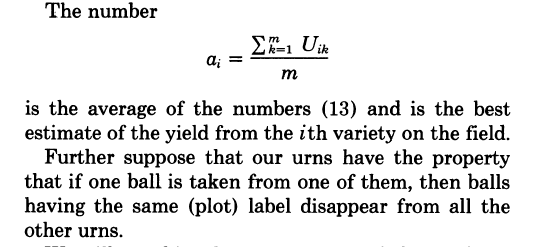
\includegraphics[height=2in]{neyman3.png}
		\label{fig:neyman3}
	\end{figure}
\end{frame}

\begin{frame}[t]\frametitle{Tickets}
	\begin{figure}[htbp]
		\centering
			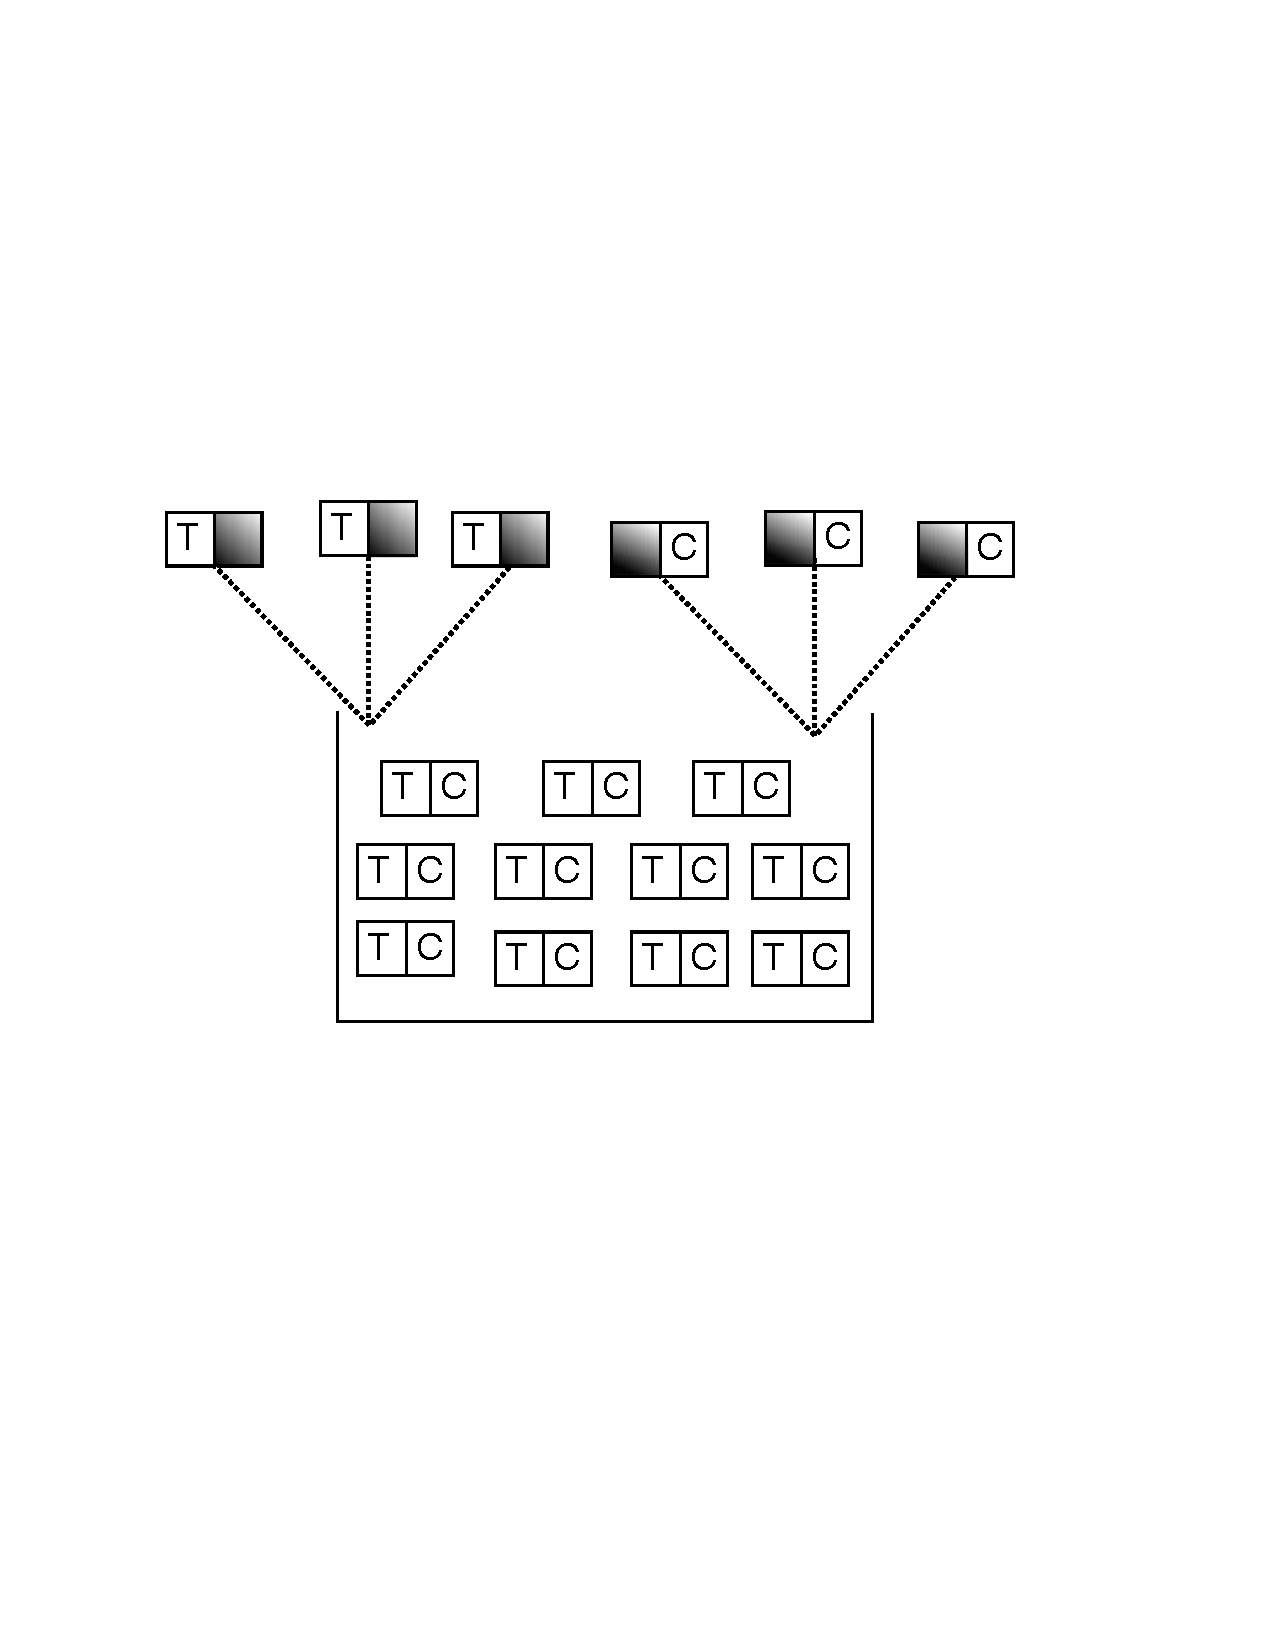
\includegraphics[height=3in]{potential_outcomes.pdf}
\		\label{fig:potential_outcomes}
	\end{figure}	
\end{frame}

\begin{frame}[t]\frametitle{A Sampling Problem?}
	\begin{figure}[htbp]
		\centering
			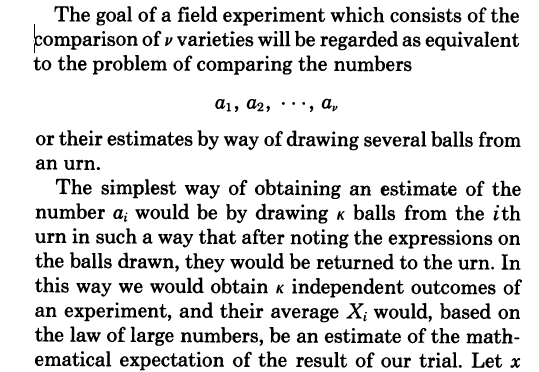
\includegraphics[height=2.7in]{neyman5.png}
		\label{fig:neyman5}
	\end{figure}
\end{frame}

\begin{frame}[t]\frametitle{Average Treatment Effects}
	\begin{figure}[htbp]
		\centering
			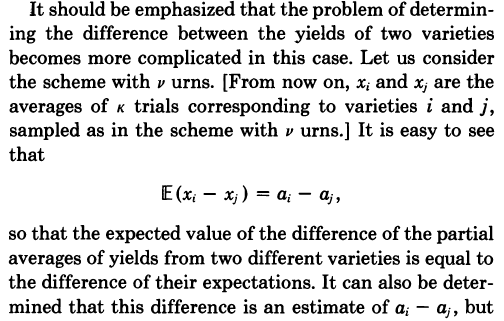
\includegraphics[height=2.5in]{neyman6.png}
		\label{fig:neyman6}
	\end{figure}
\end{frame}

\begin{frame}[t]\frametitle{Where does Uncertainty Come From?}
	\begin{figure}[htbp]
		\centering
			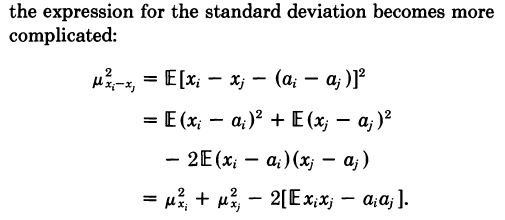
\includegraphics[height=1.7in]{neyman7.png}
		\label{fig:neyman7}
	\end{figure}
\end{frame}

\section{Causal Effects} % (fold)
\label{sec:modern_notation}
% section modern_notation (end)
\begin{frame}[t]\frametitle{Defining Causal Effects}
	\small
		 \begin{tabular}{ccc}
		\hline
		Group & $Y_{i1}$ & $Y_{i0}$\\
		\hline
		 $T=1$ & Observable: $Y_{i1}|T=1$ & Counterfactual: $Y_{i0}|T=1$\\
		 $T=0$ & Counterfactual: $Y_{i1}|T=0$ & Observable: $Y_{i0}|T=0$\\
		\hline
		\end{tabular}
	\normalsize
	\vspace{.5in}
	\begin{itemize}
		\item<+-> Observed Outcome: $Y_i = T_iY_{i1} + (1-T_i)Y_{i0}$ 
		\item<+-> Individual causal effect: $\tau_i = Y_{i1}-Y_{i0}$	
		\item<+-> Estimand is ATE (SATE): $\bar \tau	 = E[Y_{i1} - Y_{i0}]$	
		\item<+-> How useful is ATE when effects are heterogeneous?  
		\item<+-> Decompose $\bar \tau$:
		\[ \begin{array}{rl}
		\bar \tau &=   \{\pi E[Y_{i1}|T=1] + (1-\pi) E[Y_{i1}|T=0]\} \\
		&- \{\pi E[Y_{i0}|T=1] + (1-\pi) E[Y_{i0}|T=0]\}
		\end{array} \]
		, where $\pi$ is the proportion in the treatment group.		
		\end{itemize}
	\end{frame}
	\begin{frame}[t]\frametitle{Identifying $\bar \tau$}
		\begin{itemize}
			\item<+-> $\pi$, $E[Y_{i1}|T=1]$, and $E[Y_{i0}|T=0]$ are estimable from data, but $E[Y_{i1}|T=0]$ and $E[Y_{i0}|T=1]$ are not.
			\item<+-> Expected bias:
			{\footnotesize 
				\[ \begin{array}{rl}
				E[Y_{i1}|T=1]- E[Y_{i0}|T=0] &=  \bar \tau + \{E[Y_{i0}|T=1] - E[Y_{i0}|T=0]\} \\
				&+(1-\delta) \{E[\bar \tau|T=1] - E[\bar \tau|T=0] \}
			\end{array} \]}
			\item<+-> $\{E[Y_{i0}|T=1] - E[Y_{i0}|T=0]\}$ is \emph{expected baseline bias}, difference in the average outcome in the absence of treatment. 
			\item<+-> $(1-\delta) \{E[\bar \tau|T=1] - E[\bar \tau|T=0] \}$ is \emph{differential treatment effect} bias, i.e. the average difference in the treatment effect between those in the treatment group and those in the control group.
		\end{itemize}		
	\end{frame}

\begin{frame}[t]\frametitle{Identifying Assumptions}
	What assumptions do we need to identify $\bar \tau$?
	\begin{itemize}
		\item Assumption 1: $E[Y_{i1}|T=1] = E[Y_{i1}|T=0]$
		\item Assumption 2: $E[Y_{i0}|T=1] = E[Y_{i0}|T=0]$
	\end{itemize}
	A global assumption that gets us both assumption 1 and assumption 2 is independence between treatment assignment and potential outcomes:
	$$\{Y_{i1},Y_{i0}\}\independent T$$
\end{frame}

\begin{frame}[c]\frametitle{Beyond ATE}
	What about other estimands?
	\begin{itemize}
		\item<+-> Average effect of treatment on the treated (ATT): $\bar \tau|(T=1) = E[Y_{i1}|T=1] - E[Y_{i0}|T=1]$
		\item<+-> Average effect of treatment on the controls (ATC): $\bar \tau|(T=1) = E[Y_{i1}|T=0] - E[Y_{i0}|T=0]$		
	\end{itemize}
	\end{frame}

\begin{frame}[t]\frametitle{Selection on Observables}
	\begin{itemize}
		\item<+-> Conditional independence:
		$$\{Y_{i1},Y_{i0}\}\independent T|X$$
		\item<+-> With this assumption, it follows that:
		\begin{itemize}
			\item  $E[Y_{i1}|T=1,X] = E[Y_{i1}|T=0,X]$
			\item  $E[Y_{i0}|T=1,X] = E[Y_{i0}|T=0,X]$
		\end{itemize}
		\item<+-> If we are interested in ATT, we only need the following:
		\begin{itemize}
			\item  $E[Y_{i0}|T=1,X] = E[Y_{i0}|T=0,X]$
		\end{itemize}
		\item<+-> If we are interested in ATC, we only need the following:
		\begin{itemize}
			\item  $E[Y_{i1}|T=0,X] = E[Y_{i1}|T=1,X]$
		\end{itemize}
		
	\end{itemize}	
\end{frame}

\begin{frame}[c]\frametitle{ATT}
	\begin{figure}[htbp]
		\centering
			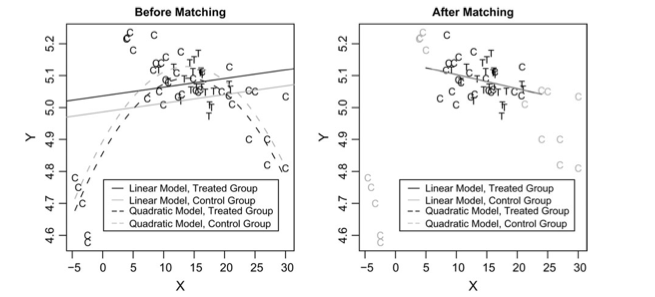
\includegraphics[height=2in]{imbalance.png}
		\label{fig:imbalance}
	\end{figure}
	
	
\end{frame}
\section{SUTVA}	
	\begin{frame}[t]\frametitle{SUTVA}
		\begin{itemize}
			\item<+-> SUTVA: ``Stable Unit Treatment Value Assumption''
			\item<+-> Rubin: ``SUTVA is simply the a priori assumption that the value of Y for unit $u$ when exposed to treatment $t$ will be the same no matter what mechanism is used to assign treatment $t$ to unit $u$ and no matter what treatments other units receive.''
			\item<+-> ``No interference between units'' is  ``the observation on one unit should be unaffected the particular  assignment of treatment to the other units''
		\end{itemize}
	\end{frame}
	
	\begin{frame}[t]\frametitle{No Interference}
		\begin{itemize}
			\item Consider a uniform randomized experiment with two strata, four units in the first strata and two units in the second strata, for 6 units in total. Half the units in each stratum receive treatment. 
			\item There are 12 possible treatment assignments contained in the set $\Omega$.			
		\end{itemize}
		\begin{figure}[htbp]
			\centering
				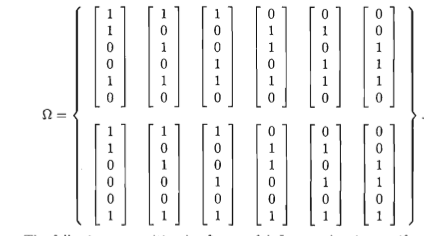
\includegraphics[height=1.5in]{omega.png}
			\label{fig:omega}
		\end{figure}		
	\end{frame}
	
	\begin{frame}[t]\frametitle{Causal Effects without SUTVA}
		\begin{itemize}
			\item Without SUTVA, a causal effect is defined for every possible combination of the treatment assignment.
			\item The potential outcome for unit $i$ might be $Y_{i100000000000}$ or $Y_{i010000000000}$, etc. 
			\item How many potential outcomes will each unit have? 
			\item Potential outcomes still well defined! 
		\end{itemize}
	\end{frame}

\end{document}
